\documentclass{standalone}
% preamble: usepackage, etc.
\begin{document}

\chapter{相关技术和理论}
近些年来,人工智能的发展非常迅速,经历了几个不同的阶段。从最开始计算智能
到感知智能的阶段,正在迈向认知智能的阶段\citing{sunli2018ren,wangqin2019ren}。
但要实现认知智能,
第一步是如何让机器学会理解人类复杂语言中所包含的语义,在理解自然语言的语义
基础上,进而对已有的知识做逻辑推理,无论是传统的规则演变还是深度学习的手段,
如何将深度学习与逻辑推理相结合是人工智能当前所面临的难题。目前深度学习在自然
语言处理中的命名体识别、关系抽取均取得不错的效果,知识图谱是一种表征自然语言
语义的很好的载体,在知识图谱的基础上做知识演变、逻辑推理是当前研究的热门方向。
\section{知识图谱}
\subsection{知识图谱概念}
知识图谱这个概念最早是由谷歌在2012年正式被提出,当初提出知识图谱概念
是为了优化谷歌搜索引擎的搜索效率,缩短响应时间。用图的形式存储知识,
从而代替传统基于关键词的文本数据。事实上,知识图谱的起源可以追溯到更早的
上世纪60年代的语义网络,经过长达半个世纪的发展和演变,才有了如今知识图谱
完整的表示。1960年Quillian首次提出表示知识的全新模式,即语义网络,用网络
中的点表示概念、事物、对象等,网络中的边表示概念实体之间的关系。尽管这种知识
表示模式很快得到大家的接受,非常直观简洁,但是很难应用到实际场景,主要原因
在于网络中的节点和边完全用户自定义,过于随意,没有统一的规范和标准,因此
很难去编码。

到80年代左右,相继出现本体论(Ontology)和万维网的概念。本体论可以
理解成一种计算机模型,用于描述抽象实体或者概念、关系以及属性之间所
组成的知识结构模型,基于此知识结构模型可以去进行知识推理。1989年
Time Berners-Lee发明了万维网,实现了文本间的链接。万维网通过超文本标记语言(HTML)
将超文本链接从一个站点跳到另个站点\citing{wang0shu}。
1999年万维网之父Tim Berners-Lee提出了语义网(Semantic Web)的概念\citing{liu2006ben,
hao201ji},
语义网可以理解为在万维网的基础上对数据进行了粒度降解处理的一种
网络流通的通用框架模型。将以往基于document的数据格式碎片化
成更小的数据源data,这些数据源data同样构成一个庞大的信息网络,
因此如何去在不同的data之间信息传递和链接时语义网研究重点,即
linked Data,对于不同的信息源,将其从page或者document转换成
Data的数据格式,并将这些数据作为公开数据集,为了保证网络流中
每个data的规范性和唯一性,通常参考已知本体进行建模并赋予data一个URI
进行标识。

知识图谱在知识表示上具有天然优势,形式上以图的形式表示客观世界中的
实体以及实体之间的关联,其中这些实体是由概念、事物、人、对象组成。
这些实体和关系可以用最小的表示形式去建模,即三元组结构。三元组结构
可以表示两个实体之间的关联,这两个实体可以是相同实体,也可以是不同
实体。例如人属于灵长类生物,这句描述的三元组建模结构是<人,属于关系,灵长类生物>。
三元组在图谱中的呈现形式就是对应两个点,关系则是它们之间的边。
相对于传统的语义网而言,它的数据粒度变得更小,更见直观的表示实体本身,
这样完成了文档或者网页的超链接万维网到实体于实体之间关系互联的转变。
这种转变不仅仅是数据粒度变得更小,知识图谱引擎除了提供类似传统的查询、搜索
、字符集匹配等基本功能外,它包含了更深层次的语义知识。因为之前的文本
首先会经过自然语言理解,抽取实体以及它们之间的关系,然后在利用知识图谱
进行表征。因此用户进行人类语义查找时,其实会有自然语言理解之后对应的
实体关系,知识图谱中显示出所有同义和关联的语义实体。因此,知识图谱
积聚了传统知识搜索知识表示模型的优点,同时又具有自身特色,它庞大的网络关系图可以表示很复杂的语义知识,
通过对网络中的实体和关系查询可以显示出它们的内在联系。

随着移动互联网技术的飞速发展,人们每天浏览新闻、社交网络、电子消费等
会产生海量数据,如何快速的进行信息检索,精准的信息推送背后都必定
有庞大的知识图谱作为支撑。金融知识图谱,医疗知识图谱,教育知识图谱
均在行业内发挥着知识承载的作用,虽然知识图谱应用已经十分广泛,有些应用已经开始产品化,但不能忽视知识图谱
带来的问题和面临的挑战。知识图谱目前面临的挑战包括三个方面。第一方面,是
知识图谱构建的问题。不同领域知识图谱
对构建的标准很高,只有行业内专家才能构建出准确、完整的知识图谱,但是缺点也是
显而易见的,人工成本过高,而且耗时效率低下。所以如何自动或者半自动构建
知识图谱成为研究重点。第二方面,知识图谱与深度学习相融合。对于急剧增加的
海量数据,传统搜索图搜索算法效率会下降明显,需要利用深度学习去处理图数据。
图嵌入、图编码、图匹配等一系列问题需要考虑。第三方面,图上的逻辑推理。
知识图谱与逻辑推理结合是目前的难点,如何在图的节点之间体现逻辑关系,以及
图节点如何引入计算都还处于研究阶段。
\subsection{知识图谱模型}
知识图谱的构成主要指从数据模型的角度分析,它包含数据层(data layer)和模式层(schema layer)两个部分。
其中,模式层是知识图谱底层的概念存储,是数据模型的核心组成部分\citing{huangyu2019zhi,
zhouli2019ji}。主要是
本体概念和概念之间的关系构成的。这些概念实体可以理解成对上层数据层的
具体实例化实体和关系一种规范化约束,因此数据层与模式层是一种依赖约束关系。
模式层约束着数据层,而数据层由同样看作模式层本体的实例化结果。在一些只承担
搜索查询的知识图谱中,通常只需构建数据层节点和关系即可。模式层在推理知识图谱
中有着重要应用,它可以从本体的约束关系中构建相对应的抽象实体类和抽象关系类,
同时模式层采用的树状类结构,类之间的继承关系可以在Java中类继承保持一致性,方便编码工作。
关系是有向性,有向性分为单向有向性和双向有向性。关系中可以存储属性,同样关系也可以
有继承结构。

在数据层,是具体模式层的本体和关系的实例。对于每一组的实体和关系实例,可以用三元组
结构<实体-关系-实体>去描述。所有的三元组结构组织成了关系图,值得注意的是,三元组中的
实体和关系还可以存储属性,例如数学表述“点P到直线l的距离为d”,解析成的三元组结果
为<点,距离关系,直线>,而“距离”作为距离关系的属性,属性值为d,属性无论是在实体
或者关系中的存储都是key-value键值对的方式。对于属性的存储与三元组存储可以相互转换,
上述例子中“距离”可以单独视为一个实体-距离实体,这样便完成<实体-属性-属性值>到
<实体-关系-实体>的转变。


如图2-2所示是知识图谱数据模型的构成图实例。
\begin{figure}[htbp]
	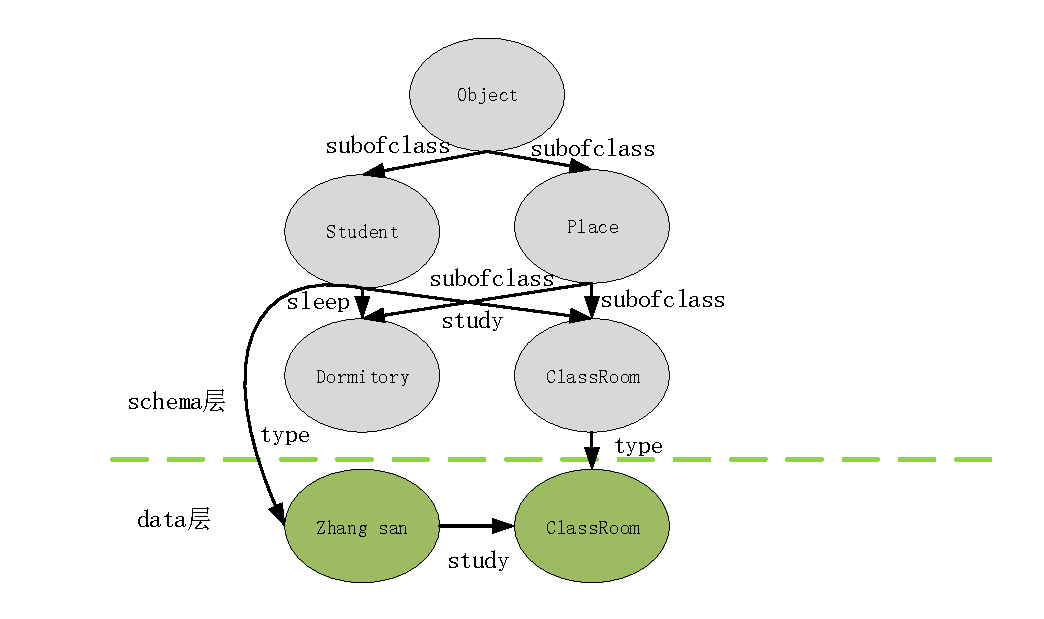
\includegraphics{知识图谱模型构成.pdf}
	\caption{知识图谱构成图实例}
	\label{知识图谱模型构成}
\end{figure}
\subsection{知识图谱构建}
通过上一章节对知识图谱的构成介绍可知,知识图谱的数据模式包含模式层和数据层,
二者的依赖关系是模式层是顶层架构,而数据层是底层应用,是模式层的具体实现。
从构建的方向可以分为两种构建方式,自底向上和自顶向下\citing{zhangyin0ji,chuyinzhi}。
自底向上的构建方式
是先从不同的数据源中抽取实体、关系、属性等知识,然后将知识添加到知识图谱
的数据层形成三元组结构\citing{zhangjie0wen,macan0mian},当形成的三元组知识逐渐丰富时,对知识图谱中的实体
关系进行分类、归纳、整合处理,抽象成顶层的本体和关系结构。因此自底向上
是先数据层后模式层构建的方式。自底向上的应用场景主要是大型的共有库构建,
因为大型共有库构建是所有人都可以参与,知识来源形式多样、知识表述多元化,
这样的知识库很难在最初的时候确定模式层的本体和关系结构,只有通过不断的
累积数据然后再去抽象数据共性成概念本体。自顶向下则是相反的构建思路,
先构建好所有本体以及本体间的关联,然后再根据数据源去构建数据层,在顶层
约束下对数据层进行规范化、标准化构建本体实例和关系。这种构建模式一般
应用于行业内的知识图谱,知识图谱的规模有限,构建的知识图谱质量高,但缺陷在于需要专业人士才能
构建并且使用范围有限。因此,当前正在积极探索将二者相融合的构建方式,发挥各自的
优点。

在明确知识图谱的构建方式后,数据来源和具体构建流程问题是构建的重点。
数据来源是构建知识图谱的首要问题,不同的数据源会有不同的数据结构,因此
需要对数据进行分类处理,不同类采用不同的构架方式。通常情况下,按照
数据结构化程度将数据分为三种:结构化数据、半结构化数据和非结构化数据\citing{shencao2019ji}。
结构化数据具有数据结构清晰、界限明确、格式规整的特征,多为关系型
数据库中存储的数据\citing{yufang2019da},对于结构化数据通过D2R技术转换成RDF(linked data)格式的数据,
D2R是由D2R Server,D2RQ Engine和D2RRQ Mapping语言三个部分组成。D2R Server
可通过HTTP请求提供外部查询的接口访问服务,主要是可供浏览器调用或客户端调用。
D2RQ Engine主要功能是将D2RRQ Mapping文件转换成RDF格式\citing{liyou0ji,
chncan2018ji},是基于jena(一种语义网的Java平台)
的接口。D2RRQ Mapping是将关系型数据的结构化数据虚拟映射成RDF数据格式的Mapping规则集。
相对于结构化数据,半结构化数据来源更加广泛,例如网页中的数据、百科的数据,这些数据都具有
有相对结构的数据,但又不能直接使用需要进一步处理。对于半结构化数据,可以使用传统的正则
表达式去匹配然后转换成结构化的数据,再利用结构化数据转RDF格式的相关技术处理,当数据集
有一定规模时,可以采用有监督学习的方法在有标注的训练集上学习抽取规则,再去新的网页数据抽取。
实际情况最普遍的数据格式是非结构化的,人类的语言就是典型的非结构化数据。处理非结构数据的
第一步需要借助自然语言理解,命名体识别和关系抽取,将非结构化数据的语义特征转变成三元组结构。

知识图谱具体构建流程由四个部分组成:原始数据、知识抽取、知识修正、数据模型规范。知识
修正主要处理同一实体多个类型以及隐含实体指代消解问题,是自然语言理解的语义理解修正。
数据模型规范是构建知识图谱的模式层,顶层设计来约束底层的数据层数据标准化。如图2-3是
知识图谱的构建流程图。
\begin{figure}[htbp]
	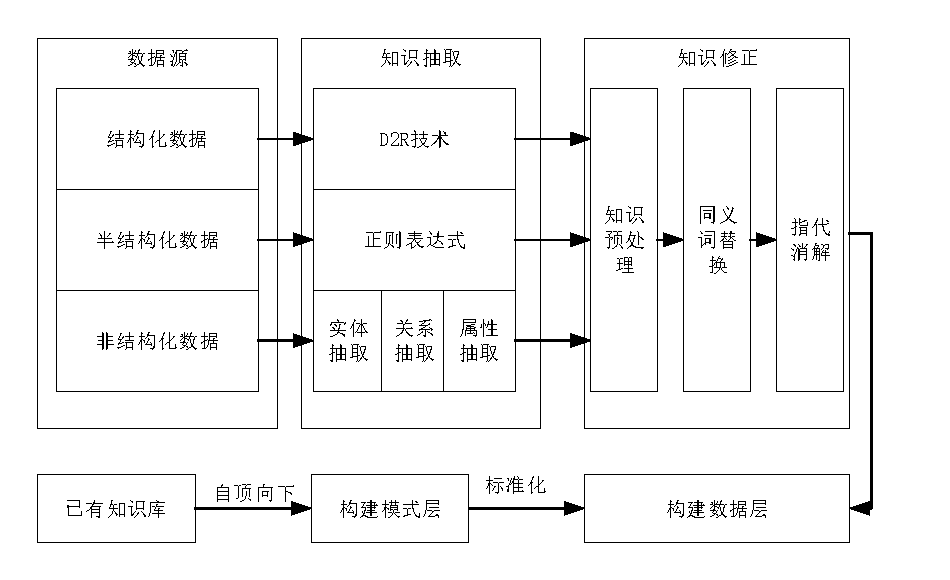
\includegraphics{知识图谱构建流程图.pdf}
	\caption{知识图谱构建流程图}
	\label{知识图谱构建流程图}
\end{figure}
\section{图数据库}
\subsection{图数据库概述}
在完成原始数据到知识图谱构建之后,需要考虑以什么方式去存储知识。
一种是基于关系型数据库进行存储,一种是基于图数据库存储。关系型数据存储是
将知识图谱转换成RDF三元组<Entity,Relation,Entity>进行存储\citing{zhangzhao2019ji},RDF存储的
优势在于利于共享和发布数据,但RDF三元组存储时会丢失属性信息。基于图数据库
存储是以图作为基本模型,图中的节点和边分别存储实体和关系信息,同时图数据中的
节点和边都可以存储其属性信息,图数据库在查询和搜索效率是高效的,也可以表示
复杂的语义知识,对知识图谱的显示作用也更好,其次,传统的关系型数据
是以表的形式存储数据,对查询关联数据需要不断联表查询,效率较为低下,而图
数据库对关联查询友好支持,整体来说更适合作为知识图谱的存储。如表2-1所示
图数据库与其他类型数据库的对比。
\begin{table}[h]
	\caption{不同类型数据库对比} 
	\begin{tabular}{|c|c|c|c|} 
		\hline  
		数据库类别 & 数据存储结构 & 特点 & 实例 \\
		\hline 
		图数据库 & 图 & 知识表示间接直观,关系查询高效 
		& Neo4j\\  
		\hline  
		关系型数据库 & 数据表 & 数据以行和列的方式存储在表中,支持联表查询 
		& Mysql\\  
		\hline  
		键值数据库 & 哈希表 & 一般直接存储在内存,查找速度快
		& Redis \\  
		\hline 
		文档数据库 & 键值对扩展 & 非结构化直接对文档插入数组数据
		& MongoDB\\  
		\hline 
	\end{tabular}
	\label{tablea}
\end{table}
图数据库近些年来之所以得到广泛的认可,最主要的原因在于它在不同的应用场景中
相对于传统的数据库在知识表示、搜索查询、关联查询都有明显的效果提升。现在
越来越多的领域都在构建知识图谱,搜索领域,谷歌最早就用知识图谱做搜索优化,
后面国内的百度百科也开始构建共有知识库;社交领域,FaceBook,Twiiter等社交
平台利用知识图谱进行好友推荐,新闻推荐;零售领域,ebay,沃尔玛使用它进行
商品的实时化和个性化推荐,提升用户购买体验。另外,图数据因为其表示形式
简洁直观也是受到青睐的原因之一。它利用图数据结构来存储客观时间的语义知识,
图可以看作是点集和边集的组合,其中节点是图数据库主要数据元素,边是连接不同
节点之间的关系。
\subsection{图数据库Neo4j}
当前市面的图形数据库百花齐放,目前Neo4j以绝对的优势成为最受欢迎的图数据库。Neo4J是
Neo Technology所提供的基于Java实现的开源图形数据库\citing{qufeng2018ji}。Neo4J与其他数据库一样支持事物以及
事物的ACID四大特性,同时Neo4J的专业版支持集群和主从复制。Neo4J之所以能
够表示复杂语义,主要是依赖其图模型。图模型从标签、节点、关系、属性四个
方面入手。标签是对节点和关系作为分组的一种标识,可以提高查询的速度和
分类管理。一个节点和一条关系可以拥有一个标签,也可以是多个标签,依据标签索引
便可得到同标签的所有节点和关系;节点存储知识抽取中的概念实体,Noe4J的节点支持
属性以key-value键值对存储,节点中的属性可以是一个或者多个;边存储的是实体之间
的关系,表示方式是有向边,与实体一样关系也支持属性存储;对于属性的存储Neo4j
只支持键值对存储,属性可以被索引和查询。Neo4J目前支持的数据格式有整形常量,
字符串以及字符串数组,不支持对象存储,当属性是对象时就会出现无法兼容的情况。

Neo4J作为一种图数据库有自己的查询语言和语法,Cypher是Neo4J官方提供的
图形查询语言,单个Neo4J实例可以存储几十亿的节点和关系数据,它的查询功能非常强大,
是汲取各种数据库查询语言的思想并应用在图上查询。Cypher是一个申明式的语言\citing{lvdan0ji}。
Cypher查询语言常用关键字“match”、“create”、“where”、“filter”、“project”
等用于条件过滤查询,Neo4J同时提供了相关的操作函数,可用于节点查询、字符串处理等。

Neo4J为了支持更强大的图查询和图重构功能,它还支持各种
插件功能,APOC是Neo4J后续版本中提供的过程调用包,这些过程调用函数是Java实现的,
可以直接部署到Neo4J实例里面包含丰富的过程调用和复杂图查询算法,如下表2-4所示
是APOC常见图算法过程调用。 
\begin{table}[h]
	\caption{部分APOC过程调用} 
	\begin{tabular}{|c|c|c|} 
		\hline  
		过程调用 & 参数 & 功能描述\\
		\hline 
		apoc.path.expand() & \makecell[l]{startNode <id>|Node, \\relationshipFilter, labelFilter,\\ minLevel, maxLevel} 
		& 路径扩展 
		\\  
		\hline  
		apoc.path.subgraphNodes() &\makecell[l]{startNode <id>Node/list,\\maxLevel, relationshipFilter, labelFilter,\\ bfs:true,limit:-1, optional:false} 
		& 在子图中扩开节点 
		\\  
		\hline  
		apoc.path.subgraphAll() & \makecell[l]{startNode <id>Node/list,\\maxLevel, relationshipFilter, labelFilter,\\ bfs:true, filterStartNode:true, limit:-1} 
		& \makecell[l]{扩展子图 \\并返回所有子图路径}
		\\  
		\hline 
		apoc.algo.dijkstra() & \makecell[l]{startNode, endNode,\\'KNOWS|IS\_MANAGER\_OF>',\\ 'distance'} 
		& dijkstra算法搜索最短路径算法
		\\  
		\hline 
		apoc.algo.aStar() & \makecell[l]{startNode, endNode,\\'KNOWS|IS\_MANAGER\_OF>',\\ 'distance','lat','lon'} 
		& A*算法搜索最短路径
		\\  
		\hline 
	\end{tabular}
	\label{tablea}
\end{table}
\section{自动推理}
\subsection{产生式系统}
产生式系统是人工智能认知模型中最典型的体系结构之一,其最核心的思想通过依据产生式规则
对已知事实进行推理演变,从而产生更多的知识,将新生成的知识重新加入到已知事实库中,然后继续迭代。
从核心思想可以总结出产生式系统的逻辑结构,首先是已知事实,由于已知事实的输入需要转化成计算机
能够理解的知识,便涉及到知识表示问题;其次是产生式规则,产生式规则的基本形式是“<If P,then Q>” \citing{chenopin2003ji},
其中P代表规则的前提条件集合,Q的含义分为两种:动作或者结论。当Q表示动作时,意味着当满足P条件时,
规则会触发相对应的动作;当Q代表结论,则在满足所有前提条件时,会生成结论知识。最后是产生式系统的
控制策略,控制策略负责对整个系统进行流程控制、策略调度、规则选取及应用、动作执行等。如图2-4是产生
式系统模块图。
\begin{figure}[htbp]
	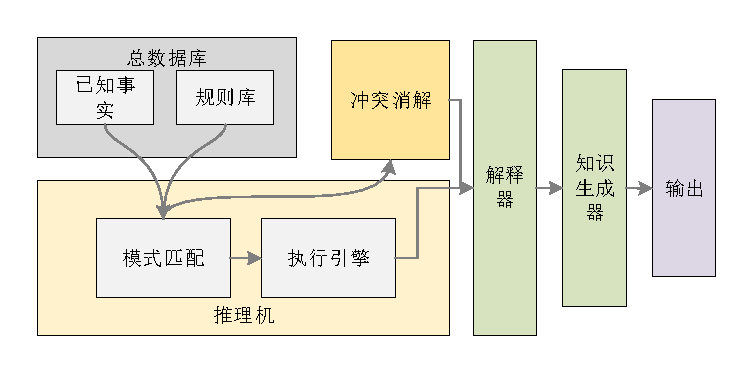
\includegraphics{产生式系统.pdf}
	\caption{产生式系统结构图}
	\label{产生式系统}
\end{figure}
逻辑推理的三种推理方式:正向推理、逆向推理和正逆结合,均可适用于产生式系统。具体工程中
会根据实际情形选取不同的产生式系统,正向推理的产生系统是一种暴力搜索思想,适用规则库
规模中等的系统,若规则库规模过大,会产生知识爆炸问题,下面详细阐述正向推理的算法过程:

1)首先将已知事实经过知识抽取,自然语言理解成计算机表示的知识,全部放入知识库中。

2)读取知识库中已知事实,将已知事实"(conditions,askings)"划分成前提条件C和求解目标A两个部分。

3)在规则库选取规则,将产生式规则“<If P,then Q>”划分成前提条件P和结论或者动作Q两个部分。

4)将步骤2)中已知事实前提条件C与步骤3)中产生式规则P进行匹配,若匹配成功,执行步骤5),
若匹配失败,回溯到算法的步骤3)执行。

5)将产生的新知识与步骤2)中已知事实求解目标A进行匹配,若匹配成功,则结束正向推理,推出;
若匹配失败,执行步骤6)。

6)将新知识插入到已知事实库中,若插入成功,回溯到算法的步骤3)执行;若插入失败,
进入知识冲突消解策略。

与正向推理的盲目式搜索不同,逆向推理的前提是已知事实中求解目标明确,逆向推理的核心
思想就是分解子目标,然后再去不断规约子目标,直到到达所有满足条件的事实,终止规约。
下面详细阐述逆向推理的算法过程:

1)首先将已知事实经过知识抽取,自然语言理解成计算机表示的知识,全部放入知识库中。

2)将已知事实中的求解目标分离,构建规约树的根节点。

3)利用分支技术分解求解目标节点,生成多个子目标。

4)去规则库中寻找子目标对应的产生式规则,若能够找到对应规则,执行步骤5);
若找寻失败,回溯到算法步骤3)。

5)将产生是规则的前提条件分解出来,若所有的前提条件都存在已知事实,停止规约,执行步骤6);若
存在某个前提条件不存在已知事实,继续规约,回溯到算法步骤3)。

6)遍历规则的规约树,生成规则路径。

从上文的正向、逆向两种算法可以看出,无论哪种推理方式,都需要规则库的支撑。
尽管产生式系统逻辑结构清晰,模块化独立程度高,也适用多种推理方式,但也有
自身的缺陷和不足。最主要的问题在于当规则库规模过大时,系统缺陷就会比较明显,
规则数量多是会对匹配的精度要求高,每一个规则都需要经历同样的推理流程,时间消耗
较大,产生的知识越多,继续迭代会产生知识爆炸,同时知识冲突的概率也会急剧增加。
因此针对这些问题,需要引入知识减枝的策略和知识冲突消解的策略。
\section{匹配算法}
基于规则的推理引擎,其核心算法思想就是匹配算法,通常情形下,匹配算法是对已知事实
与待匹配事实搜寻验证的过程。由于不同规则库知识表示的有所差异,决定了
匹配算法设计是不同的,主要根据产生式规则和实例化知识图谱规则将匹配算法
分为两大类:模式匹配和图匹配。
\subsection{模式匹配算法}
模式匹配是指将已知事实与知识库进行匹配,从匹配对象类型可以分为字符串匹配,类对象匹配,或者
规则匹配,三种模式匹配的主要区别在于匹配粒度,其中规则匹配粒度最粗,字符串的匹配粒度最细。
另外类对象匹配和规则匹配依赖于字符串匹配,本文中引擎的匹配算法是融合三种模式匹配方式,
能够处理较为复杂的匹配搜索问题。规则匹配相对于字符串匹配
较为复杂,首先定义规则条件部分(left-hand side),简称LHS,结论部分(right-hand side),
简称RHS。规则分为条件和结论两部分,条件部分参与事实匹配,结论部分可以产生新知识,
而事实集满足匹配条件的前提是包含所有规则集条件。具体的算法流程如下:

1)将选取的实例化规则R,构建条件集LHS和结论集RHS。

2)从已知事实集中构建出等价于条件集LHS同等大小的事实子集C。

3)若已知事实集C满足LHS(R)=true,则将已知事实子集C和对应规则R加入到冲突集;
否则,执行步骤4)。

4)对于M个事实选取别的组合构成新的事实子集C1,若没有新组合,执行步骤5);
否则,回溯到算法的步骤3)。

5)去规则库选取新的规则R1,执行步骤2)。 

关于模式匹配算法最为常见的有Rete算法、Tread算法、Leaps算法,这三种算法都是
前向规则快速匹配算法,递进式推理的特点是所有的动作都是串行执行的,匹配动作是最先完成的,
依据匹配动作的结果去执行实例化规则的选取动作,然后再去不断去循环之前的动作。其中,rete算法
应用最为广泛,很多规则推理引擎都直接借鉴于其中的思想。Rete算法包含两个部分,规则编译和构建rete网络,
已知事实可以在rete网络图中流动。rete具体算法过程如下:

1)将已知事实F加入到工作内存working memory

2)将已知事实F于规则库选取的规则R进行模式匹配,若匹配成功,将事实加入
到匹配元素表;否则执行步骤3)

3)激活多个规则,并将规则放入到冲突集中

4)解决冲突,将冲突的规则按照先后顺序放入到Agenda 

5)引擎去执行Agenda中的规则,重复步骤2-5),直到所有Agenda所有规则执行完毕。

\subsection{图匹配算法}
图匹配是个经典的图上匹配问题,图匹配问题涉及二分图匹配、最大连通域匹配、
子图匹配等问题。本文设计的图匹配引擎采用的算法思想就是子图匹配算法,又
称子图同构算法。所谓子图同构任务,即给定一个target graph A(m,n),和
一个query graph B(p,q)。其中,m、p是点集,n、q是边集。试图寻找一种
映射关系,使得两个图对应的点的节点类型相同,query graph中的边在target 
graph中对应的点之间都存在,节点名称可以不同,且节点类型相同。如下图3-4所示,两个
实例化子图是同构图:
*****************

本文设计的图匹配算法是依赖于知识图谱实现的,是三元组匹配和图路径匹配融合算法。
三元组匹配首先将图拆解成<实体,关系,实体>的三元组形式,三元组中的实体和关系
是对象匹配,只匹配类型是否一致,实体和关系类型全都匹配上,三元组匹配成功。由于
三元组匹配会丢失图中路径信息,因此路径匹配是对三元组匹配的检验,路径匹配是从三元组
中的节点出发,搜寻从该节点出发的所有关联节点,包括深度有限遍历和广度优先遍历。检测
关联节点集是否包含关系,若是包含关系,可以认为三元组严格匹配。具体的图匹配算法如下:

1)读取实例化定理图和题目知识图谱

2)将实例化图和题目知识图谱结构成三元组集合QTripleSet,RTripleSet

3)执行三元组匹配,若匹配成功,执行算法4);否则回到步骤2)

4)执行路径匹配算法,若匹配成功,回溯到算法2),直到所有规则三元组集遍历结束;
否则推出匹配

5)步骤4)的所有三元组匹配均成功,子图匹配成功。

\section{符号计算平台}
本论文研究的课题是初等数学问题求解,初等数学中涉及到大量的数学符号计算,
因此推理引擎的推理方式中融合了计算推理。
计算推理主要来源于计算机代数系统的支撑,目前计算机代数系统的平台实现有
Matlab、Maple、Mathematica以及基于python的sympy 等。Matlab是偏向
于数学图形的绘制,在符号计算方面表现相对于其他代数系统较弱;Mathematica
是当前最强的浮点数计算平台,但由于初等数学中涉及的主要是符号计算,并且
Mathematica只提供C编程语言的接口,而引擎的构建使用的是Java语言,出现
接口不兼容的情况;结合实际的研究问题,最终选用Maple符号计算平台,既能
支撑初等数学中符号计算需求和图形绘制,同时Maple底层是基于Java虚拟机实现的,
很好的兼容Java项目接口。Maple提供了丰富的计算函数库,例如化简”simplify“、
解方程”solve“、恒等式”identity“、半代数集”SemiAlgebraic“,
分解因式”factor“,这些基础计算接口都在推理中有所应用。以上的计算函数命令集成了
高等数学算法,可以应用于初等数学的解题。但同时Maple符号计算平台也会存在一些
问题,Maple平台在计算是不支持多线程,这对并发编程支持不友好,除此之外,Maple计算函数
集成的高等数学算法,可能会导致类人解答过程的信息丢失。
\section{本章小结}
本章主要介绍了知识图谱、产生式系统、匹配算法和符号计算平台四个方面的内容。
首先对知识图谱进行发展历程以及不同时期的特点进行了回顾,然后阐述了知识图谱
的应用以及面临的挑战,介绍完知识图谱的概况后重点介绍知识图谱的数据模型结构、
知识图谱构建以及存储等问题。第二方面是介绍了本文中使用的系统模型产生式系统,
并给出了不同推理方向的产生式系统的详细算法。第三方面介绍了推理引擎中的核心算法,
从模式匹配入手,讲述了几种常见匹配算法。最后是介绍计算推理中使用的符号计算平台Maple
的基本功能,同时对比了不同数学软件之间的区别。

\end{document}